%----------------------------------------------------------------------------------------
%	PACKAGES AND THEMES
%----------------------------------------------------------------------------------------
\documentclass[aspectratio=169,xcolor=dvipsnames]{beamer}
\usetheme{SimplePlusAIC}
\usepackage{comment}
\usepackage{hyperref}
\usepackage{csquotes}
\newcommand{\code}[1]{\texttt{#1}}
\usepackage{graphicx} % Allows including images
\usepackage{booktabs} % Allows the use of \toprule, \midrule and  \bottomrule in tables
\usepackage{svg} %allows using svg figures
\usepackage{tikz}
\usepackage{makecell}
\newcommand*{\defeq}{\stackrel{\text{def}}{=}}

%Select the Epilogue font (requires luaLatex or XeLaTex compilers)
\usepackage{fontspec}
\setsansfont{Epilogue}[
    Path=./epilogueFont/,
    Scale=0.9,
    Extension = .ttf,
    UprightFont=*-Regular,
    BoldFont=*-Bold,
    ItalicFont=*-Italic,
    BoldItalicFont=*-BoldItalic
    ]

%----------------------------------------------------------------------------------------
%	TITLE PAGE
%----------------------------------------------------------------------------------------

\title[Num. Simulation of Ice Crystal Traj. \& Frag. Dyn.]{\href{https://sinews.siam.org/Current-Issue}{Numerical} Simulation of Ice Crystal Trajectories and Fragmentation Dynamics Around the XRF1 Fuselage Nose} % The short title appears at the bottom of every slide, the full title is only on the title page

\author[Moussa Diop, Tristan Soubrie, Julien Cliquet, Jean-Mathieu, and Phillippe Villedieu]{Moussa Diop, Tristan Soubrie, Julien Cliquet, Jean-Mathieu, and Phillippe Villedieu}
\institute[SIAM NEWS DECEMBER 2023]{Department of Mathematics \newline National Central University}
% Your institution as it will appear on the bottom of every slide, maybe shorthand to save space


\date{December 19, 2023} % Date, can be changed to a custom date
%----------------------------------------------------------------------------------------
%	PRESENTATION SLIDES
%----------------------------------------------------------------------------------------

\begin{document}

\begin{frame}[plain]
    % Print the title page as the first slide
    \titlepage
\end{frame}

\begin{frame}{Overview}
    % Throughout your presentation, if you choose to use \section{} and \subsection{} commands, these will automatically be printed on this slide as an overview of your presentation
    \tableofcontents
\end{frame}

%------------------------------------------------
\section{Introduction}
%------------------------------------------------
\begin{frame}{Introduction}
Why this simulation is so important?
    \begin{itemize}
    \item Icing on airplane surfaces often causes a considerable reduction in aerodynamic performance, significant unsteady flow, inconsistent probe measurement, sudden loss of engine thrust, and engine flame out. 
    \item Several aircraft incidents and dramatic accidents that pertain to ice accretion have been recorded since the onset of aviation. 
    \end{itemize}
    Water droplets that freeze on solid airplane surfaces typically cause icing. See this \href{https://www.youtube.com/watch?v=_ps7-9KfMEc}{\textcolor{blue}{video}}.
\end{frame}

%------------------------------------------------
\begin{frame}{Introduction}
    \begin{itemize}
    \item The ice crystal icing (ICI) has garnered significant research interest in recent years. 
    %Given the challenge of assessing ICI in ground testing while also meeting flight conditions
    \item The development of the simulation tools is of significant importance.
    \end{itemize}
\end{frame}

%------------------------------------------------
\section{Simulation Tool}

\begin{frame}{Simulation Tool}
    \begin{itemize}
        \item The authors employ a tool, called \href{https://aerospacelab.onera.fr/CEDRE-Software}{\textcolor{blue}{CEDRE}}, in this study. It is a multiphysics CFD code. 
        \item Two solvers are utilized:
        \begin{enumerate}
            \item \textcolor{red}{CHARME}, to simulate the aerodynamic flow field.
            \item \textcolor{red}{SPARTE}, to predict the ice particle trajectories within a Lagrangian approach. 
        \end{enumerate}
        \item This study transpires in a sequential manner, first with CHARME and then SPARTE. 
    \end{itemize}
\end{frame}

%--------------------------------------------------------------------------

\begin{frame}{CHARME: Gas Solver}
    \begin{itemize}
        \item The \href{https://aerospacelab.onera.fr/Models-Turbulent-Combustion-in-CHARME-Solver-CEDRE}{\textcolor{blue}{CHARME}} solver is used to compute the flow field by solving \href{https://resources.system-analysis.cadence.com/blog/msa2021-the-reynolds-averaged-navier-stokes-rans-equations-and-models}{\textcolor{blue}{the Reynolds-averaged Navier-Stokes (RANS)}} for a gas mixture of two species: air and water vapor. 
        \item Specifically, the authors use \href{https://turbmodels.larc.nasa.gov/sst.html}{\textcolor{blue}{Florian Menter's $k-\omega$ turbulence model}} with shear stress transport (SST) correction and perform the time integration with an \href{https://en.wikipedia.org/wiki/Backward_Euler_method}{\textcolor{blue}{implicit first-order Euler scheme}}. 
        \item Then carry out the flux calculation with a \textcolor{blue}{second-order monotonic upwind scheme} for the conservation law method and a \href{https://ui.adsabs.harvard.edu/abs/2019ShWav..29.1065T/abstract}{\textcolor{blue}{Harten-Lax-van Leer contact flux scheme}}. 
    \end{itemize}
\end{frame}

%\begin{frame}{CHARME: Gas Solver}
%    \begin{itemize}
%        \item A symmetry plane (XZ) reduces the computational domain to half of the geometry, after which we perform steady computations. The time step was $0.01$ seconds.
%    \end{itemize}
%\end{frame}


%----------------------------------------------------------------------

\begin{frame}{SPARTE: Lagrangian Particle Solver}
   \begin{itemize}
       \item \href{https://aerospacelab.onera.fr/sites/w3.onera.fr.aerospacelab/files/AL2-11_2.pdf}{\textcolor{blue}{SPARTE}} Lagrangian particle solver is used to compute ice crystal trajectories and exchange phenomena with the gas phase. 
       \item It tracks numerical particles individually from entrance to exit, either by melting, impacting walls, or leaving the computational domain.
       %along its path
       \item Particle motion affected by: drag, gravity, added mass, and Basset history forces. 
       % at high particle-to-air density ratios and small particle size gravity and Bassed forces are neglible, the particle motion is therefore only governed by the drag force. 
       \item This study utilizes the Ganser drag coefficient $C_{D}$, which accounts for non-spherical particles and is valid for high particle Reynolds numbers.
       
   \end{itemize}
\end{frame}

\begin{frame}{SPARTE: Lagrangian Particle Solver}
   \begin{itemize}
       \item Three distinct phase-change along particle trajectories: \textcolor{blue}{sublimation}, \textcolor{blue}{fusion (melting)}, \textcolor{blue}{evaporation}. 
       \item The particle-air interface's diffusive mass and heat transfer phenomena drive these three changes.
       \item Ice crystal's interaction with a wall is mainly influenced by particle size, impact velocity, and degree of melting. 
   \end{itemize}
\end{frame}

\begin{frame}{Three Impact Regimes Exist}
Depending on the ratio between the particle's kinetic energy upon impact and its surface energy: \textcolor{red}{elastic particle bouncing}, \textcolor{red}{inelastic particle}, \textcolor{red}{particle fragmentation}.
   \begin{itemize}
       \item In the first two regimes, the particle diameter remains unchanged. 
       \item Internal cracks may form in the second regime, its kinetic energy is much more reduced than in the first regime.
       \item In the third regime, we assume that the particle shatters.
   \end{itemize}
\end{frame}


%------------------------------------------------
\section{Simulation}
\begin{frame}{Simulation Setup: Flight Conditions}
    % an industrial standard research test case
 Consider \textcolor{blue}{XRF1 fuselage nose geometry}, which Airbus provided in the MUSIC-haic project. 
    % we seek to asses the ice crystals impact-models that were developed in the framework og MUSIC-haic on a representative configuration for anemometry purposes.
\begin{table}[H]
\begin{tabular}{lllll}
\hline
\multicolumn{1}{|l|}{Altitude [ft]} & \multicolumn{1}{l|}{Angle of attack [degrees]} & \multicolumn{1}{l|}{Mach} & \multicolumn{1}{l|}{Pressure [Pa]} & \multicolumn{1}{l|}{Temperature [K]} \\ \hline
\multicolumn{1}{|l|}{$34000$} & \multicolumn{1}{l|}{$2.05$} & \multicolumn{1}{l|}{$0.78$} & \multicolumn{1}{l|}{$25000$} & \multicolumn{1}{l|}{$233.15$} \\ \hline 
\end{tabular}
\caption{1. Flight conditions}
\label{Tab1}
\end{table}
corresponds to an upstream velocity of $U_x = 238.64$ m/s, $U_y = 0$ m/s, and $U_z = 8.54$ m/s. It is moving through convective wheather that involves ice crystal particles (See Table \ref{Tab2}).
\end{frame}


\begin{frame}{Simulation Setup: Flight Conditions}
   \begin{table}[H]
\begin{tabular}{lll}
\hline
\multicolumn{1}{|l|}{Mean Mass Diameter [tm]} & \multicolumn{1}{l|}{Ice Water Content [g/m$^3$]} & \multicolumn{1}{l|}{Sphericity[]} \\ \hline
\multicolumn{1}{|l|}{$336.5$} & \multicolumn{1}{l|}{$1.15$} & \multicolumn{1}{l|}{$0.579$} \\ \hline 
\end{tabular}
\caption{2. Ice crystal characteristics}
\label{Tab2}
\end{table}
The described flight point is located within the ICI envelope, which is where ice crystal accretion is most likely to appear (See Figure \ref{Fig1})
\end{frame}


\begin{frame}{Simulation Setup: Flight Conditions}
   \begin{figure}[h]
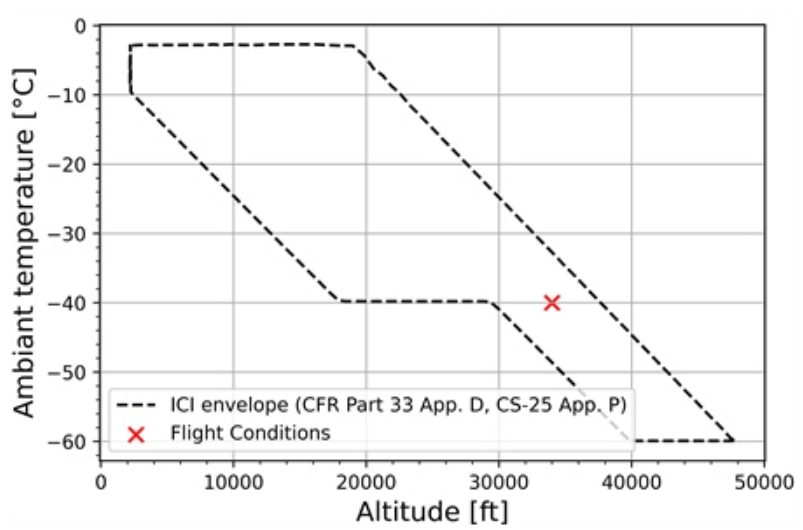
\includegraphics[width=7cm]{images/ICI_loc.png}
\caption{1. Location of flight conditions inside the CS-25 App. P envelope: A Federal Aviation Administration document that provides aircraft manufactures with the necessary requirements for aircraft certification. \textcopyright ANDHEO.}
\label{Fig1}
\end{figure}
\end{frame}

\begin{frame}{Simulation Setup: Flight Conditions}
   \begin{figure}[h]
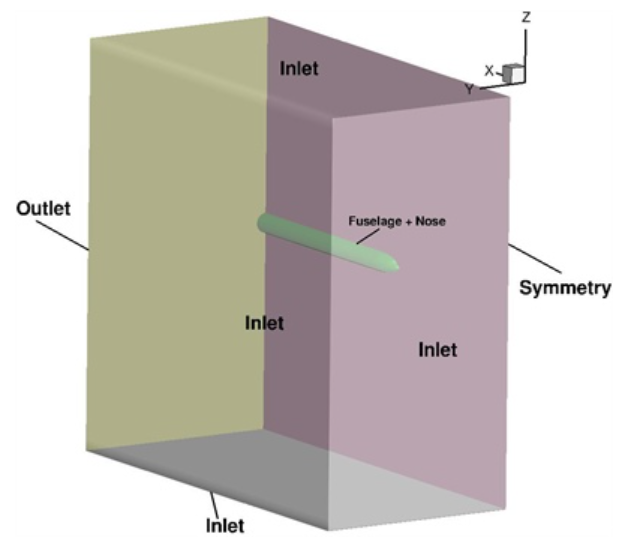
\includegraphics[width=6cm]{images/domain.png}
\caption{2.The computational domain extends to $10$ times the diameter of the fuselage upstream of the nose point in the lateral and vertical directions. \textcopyright ANDHEO.}
\label{Fig2}
\end{figure}
\end{frame}

\begin{frame}{Simulation Setup: Boundary Conditions}
   \begin{itemize}
       \item The static temperature, static pressure, and velocity are prescribed. 
       \item \textcolor{blue}{The far-field pressure} is \textcolor{blue}{25,000} pascals at the outlet. 
       \item We apply \textcolor{blue}{the non-slip condition} on walls (nose) except for the fuselage to speed up the computation. 
       \item \textcolor{blue}{Adiabatic temperature condition} is applied on the walls (fuselage and nose), to conduct the computation in a fully turbulent boundary layer. 
       \item Finally, we employ  \href{https://resources.system-analysis.cadence.com/blog/msa2021-the-reynolds-averaged-navier-stokes-rans-equations-and-models}{\textcolor{blue}{RANS}} modeling to compute the aerodynamic flow field, with \href{https://turbmodels.larc.nasa.gov/sst.html}{\textcolor{blue}{SST $k-\omega$}} as a turbulent model. 
       \item Finally, we employ  \href{https://resources.system-analysis.cadence.com/blog/msa2021-the-reynolds-averaged-navier-stokes-rans-equations-and-models}{\textcolor{blue}{RANS}} modeling to compute the aerodynamic flow field, with \href{https://turbmodels.larc.nasa.gov/sst.html}{\textcolor{blue}{SST $k-\omega$}} as a turbulent model. 
       \item Application of the turbulent $LP1$ wall function correctly estimates wall fluxes (thermal and momentum) without meshing the boundary layer's viscous sublayer. 
       %In the context of computational fluid dynamics (CFD) and turbulence modeling, wall functions are used to model the effects of a solid boundary on the turbulent flow near the wall. These functions are crucial for simulating fluid flow in situations where resolving the entire boundary layer is computationally expensive. They provide a simplified representation of the near-wall region.
   \end{itemize}
\end{frame}

%------------------------------------------------
\section{Results}


%------------------------------------------------
\begin{frame}{Discussion and Results}
  Computation of the airflow with the CHARME solver shows that the computational domain's maximum temperature is $266.7$ K, far below the melting temperature $273.15$ K.\\ 
  %this not hot enought to promote particle melting
  \vspace{2pt}
  Consequently, the rest of the results focuses on particle trajectories and the fragmentation process. 
\end{frame}

\begin{frame}{Discussion and Results}
  \begin{figure}[h]
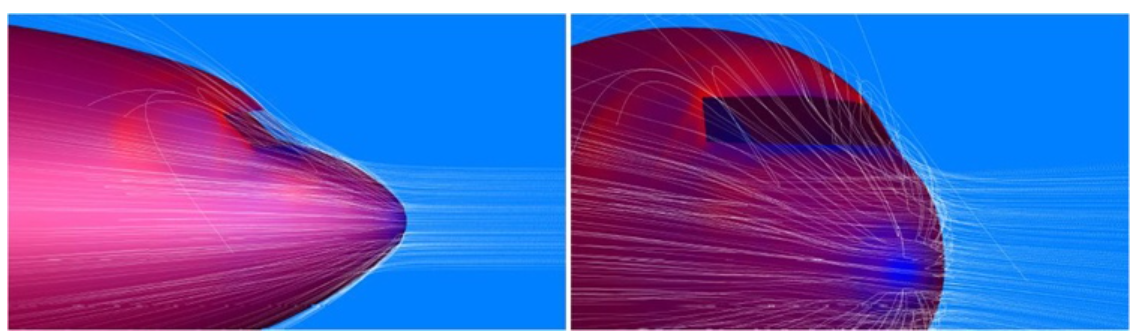
\includegraphics[width=10cm]{images/trajectory.png}
\caption{3. Particle trajectory around the fuselage. \textcopyright ANDHEO.}
\label{Fig2}
\end{figure}
Particles that arrive from the upstream position impact the nose's wall and windshield, and some deviate around the geometry (depends on particle response time).
%particle ability's to deviate around fuselage
\end{frame}

\begin{frame}{Discussion and Results}
  \begin{figure}[h]
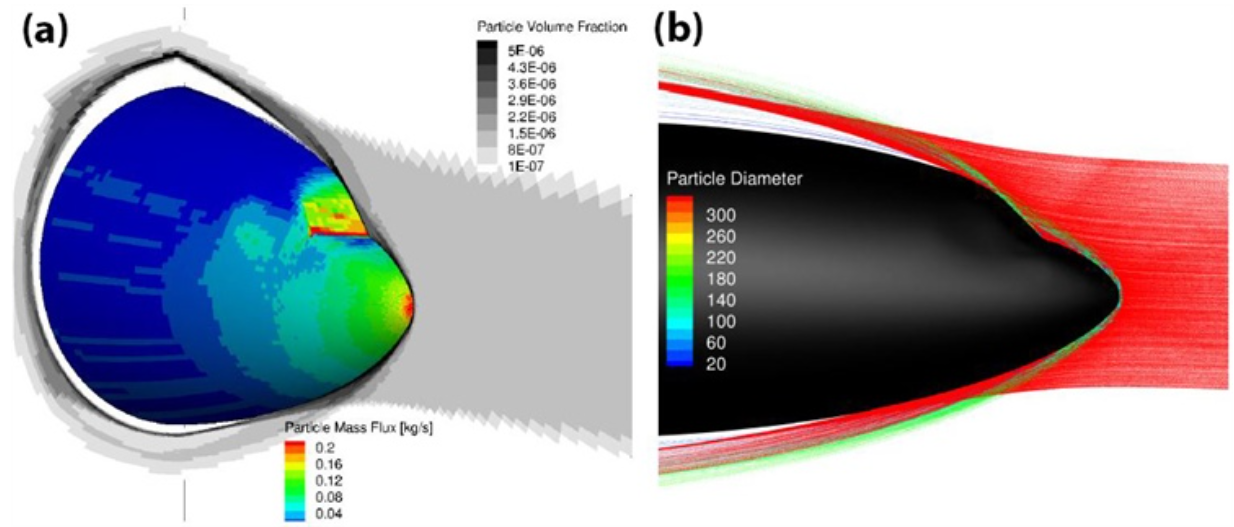
\includegraphics[width=10cm]{images/trajectory2.png}
\caption{4. Particle trajectory around the fuselage. \textbf{4a.} The particle's mass flux distribution on the fuselage. \textbf{4b.} The resulting particle fragmentation dynamics and re-emission. \textcopyright ANDHEO.}
\label{Fig2}
%The first contour illustrates the distribution of particles and highligh the particles trajectories around the fuselage. The latter indicates that particles are deflected in this area; where almost no particles go through, 
%it also highlights particle fragmentation and the remission of small-sized particles that result from fragmentation dynamics, and reveals the way in which particles move far from the wall based on their diameter.
\end{figure}

\end{frame}


\section{Conclusions}

\begin{frame}{Conclusions}
   \begin{itemize}
       \item The study examines the numerical simulation of ice crystal particle trajectories and their fragmentation upon impacting a wall surface.
       \item The authors assessed the \href{https://www.music-haic.eu/page/en/media-center/available-documentation.php}{\textcolor{blue}{MUSIC-haic fragmentation model}} in \href{https://www.onera.fr/en/site-index/computational-fluid-dynamics.html}{\textcolor{blue}{ONERA CFD software}} under real flight conditions around a fuselage nose.
       \item Results show particle deposition on the fuselage and windshield, posing icing risk with ice crystal and supercooled water droplet mix or melted particles on heated surfaces.
       \item The new model effectively captures fragmentation, assessing particle concentration near fuselage walls by considering the splitting and reinjection process.
   \end{itemize}
\end{frame}


%------------------------------------------------
\begin{comment}
\begin{frame}{References}
    % Beamer does not support BibTeX so references must be inserted manually as below
    \footnotesize{
        \begin{thebibliography}{99}
            \bibitem[Agostini A., Markwig, H., Noliau, C., Schleis, V., Sendra-Arranz, J., Sturmfels, B., 2022]{p1} Agostini A., Markwig, H., Noliau, C., Schleis, V., Sendra-Arranz, J., \& Sturmfels, B. (2022)
            \newblock Recovery of plane curves from branch points
            \newblock \emph{Preprint,} arXiv:2205.11287.
        \end{thebibliography}
        \begin{thebibliography}{99}
            \bibitem[Arzhantsev, I.V., \& Gaĭfullin, S.A., 2010]{p1} Arzhantsev, I.V., \& Gaĭfullin, S.A. (2010)
            \newblock Cox rings, semigroups and automorphisms of affine varieties
            \newblock \emph{Math. Sbornik,} 201(1), 3-24.
        \end{thebibliography}
        \begin{thebibliography}{99}
            \bibitem[Belotti, M., \& Panizzut, M., 2022]{p1} Belotti, M., \& Panizzut, M. (2022)
            \newblock Discrete geometry of Cox rings of blow-ups of $\mathbb{R}^3$
            \newblock \emph{Preprint,} arXiv:2208.05258.
        \end{thebibliography}
        \begin{thebibliography}{99}
            \bibitem[Berlow, K., Brandenburg, M.-C., Meroni, C., \& Shankar, I., 2022]{p1} Berlow, K., Brandenburg, M.-C., Meroni, C., \& Shankar, I. (2022)
            \newblock  Intersection bodies of polytopes
            \newblock \emph{Beitr. Algebra Geom.,} 63, 419-439.
        \end{thebibliography}
    }
\end{frame}

\begin{frame}{References}
    % Beamer does not support BibTeX so references must be inserted manually as below
    \footnotesize{
        \begin{thebibliography}{99}
            \bibitem[Breiding, P., \& Timme, S., 2018]{p1} Breiding, P., \& Timme, S. (2018)
            \newblock HomotopyContinuation.jl: A package for homotopy continuation in Julia
            \newblock \emph{Mathematical software – ICMS 2018,} pp. 458-465.
        \end{thebibliography}
        \begin{thebibliography}{99}
            \bibitem[Decker, W., Eder, C., Fieker, C., Horn, M., \& Joswig, M., 2024]{p1} Decker, W., Eder, C., Fieker, C., Horn, M., \& Joswig, M. (2024)
            \newblock The OSCAR book
            \newblock \emph{To be published} .
        \end{thebibliography}
        \begin{thebibliography}{99}
            \bibitem[Fieker, C., Hofmann, T., \& Joswig, M., 2022]{p1} Fieker, C., Hofmann, T., \& Joswig, M. (2022)
            \newblock Computing Galois groups of Ehrhart polynomials in OSCAR
            \newblock \emph{Sém. Lothar. Combin.,} 86B, 87.
        \end{thebibliography}
        \begin{thebibliography}{99}
            \bibitem[ Gardner, R.J., Koldobsky, A., \& Schlumprecht, T., 2022]{p1}  Gardner, R.J., Koldobsky, A., \& Schlumprecht, T. (2022)
            \newblock An analytic solution to the Busemann-Petty problem on sections of convex bodies
            \newblock \emph{Ann. Math.,} 149(2), 691-703.
        \end{thebibliography}
    }
\end{frame}

\begin{frame}{References}
    % Beamer does not support BibTeX so references must be inserted manually as below
    \footnotesize{
        \begin{thebibliography}{99}
            \bibitem[ Klartag, B., \& Milman, V., 2022]{p1}  Klartag, B., \& Milman, V. (2022)
            \newblock The slicing problem by Bourgain.  In A. Avila, M.T. Rassias, \& Y. Sinai (Eds.)
            \newblock \emph{Analysis at large: Dedicated to the life and work of Jean Bourgain,} (pp. 203-231). Cham, Switzerland: Springer Cham.
        \end{thebibliography}
        \begin{thebibliography}{99}
            \bibitem[Knuth, D.E., 1984]{p1} Knuth, D.E. (1984)
            \newblock  Literate programming
            \newblock \emph{Comp. J.,} 27(2), 97-111.
        \end{thebibliography}
}
\end{frame}
\end{comment}

%------------------------------------------------

\begin{frame}
    \Huge{\centerline{\textbf{Thank You}}}
\end{frame}

%----------------------------------------------------------------------------------------
\end{document}